\documentclass{article}
\usepackage[utf8]{inputenc}

\title{Assignment-6\\Threading}
\author{Subash Mylraj \\(CED18I051) }
\date{30 October 2020}

\usepackage{geometry}
 \geometry{
 a4paper,
 total={170mm,257mm},
 left=20mm,
 top=10mm,
 }

\usepackage{longtable}
\usepackage{graphicx}
\usepackage{listings}
\usepackage{xcolor}

\begin{document}

\maketitle

\lstset{
  language=c,
  aboveskip=3mm,
  belowskip=3mm,
  showstringspaces=false,
  columns=flexible,
  basicstyle={\small\ttfamily},
  numbers=none,
  numberstyle=\tiny\color{gray},
  keywordstyle=\color{blue},
  commentstyle=\color{dkgreen},
  stringstyle=\color{mauve},
  breaklines=true,
  breakatwhitespace=true,
  tabsize=3
}

\definecolor{dkgreen}{rgb}{0,0.6,0}
\definecolor{gray}{rgb}{0.5,0.5,0.5}
\definecolor{mauve}{rgb}{0.58,0,0.82}

\section*{Question 1: Generate Armstrong number generation within a range.}
\bigskip

\par\noindent
\textbf{\Large Code: }
\smallskip
\par\noindent\rule{\textwidth}{0.4pt}
\lstinputlisting[language=c]{src/1.c}
\par\noindent\rule{\textwidth}{0.4pt}

\bigskip
\noindent
\textbf{\Large Explanation: } \\

This program finds all the armstrong numbers from 0 to range (used input). 
Shared memory was used to store all the armstrong numbers in the range. A
structure was defined to store the array and the iterator for that array.

\bigskip
\noindent
\textbf{\Large Output:}

\begin{figure}[h]
	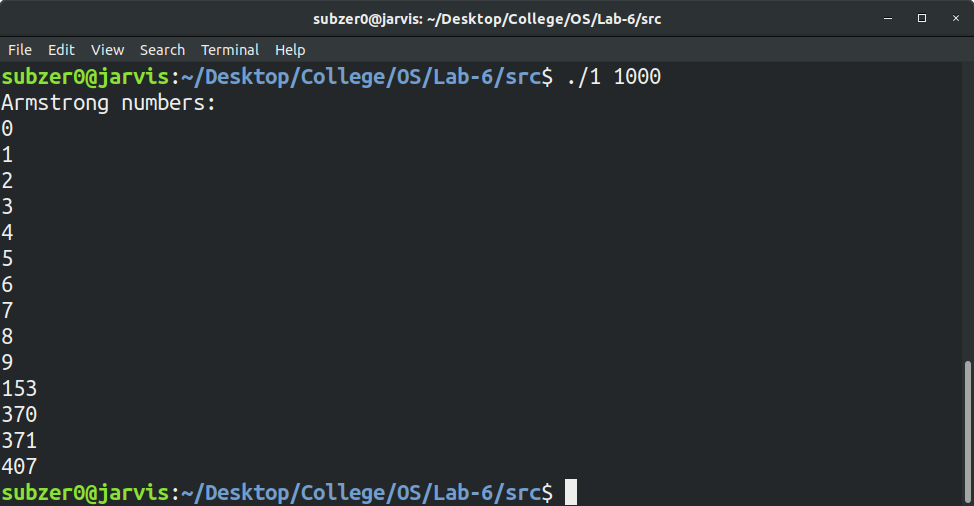
\includegraphics[width=\textwidth]{output/1.png}
\end{figure}
\bigskip


\section*{Question 2: Ascending Order sort and Descending order sort.}
\bigskip

\par\noindent
\textbf{\Large Code: }
\smallskip
\par\noindent\rule{\textwidth}{0.4pt}
\lstinputlisting[language=c]{src/2.c}
\par\noindent\rule{\textwidth}{0.4pt}

\bigskip
\noindent
\textbf{\Large Explanation: } \\

Ascending and Descending sorts are done in 2 separate threads. 
There is only one sort function which acceptsan additional 
argument for the type of sort.  The conditional statement within
the sort makes sure that bothascending and descending sorting 
can be performed.  The conditional statement resembles to the 
expression ofa multiplexor.

\bigskip
\noindent
\textbf{\Large Output:}

\begin{figure}[h]
	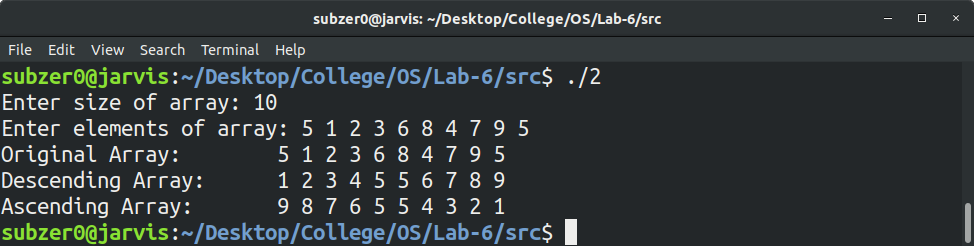
\includegraphics[width=\textwidth]{output/2.png}
\end{figure}
\bigskip


\section*{Question 3: Implement a multithreaded version of binary search. By default, you can implement a search for the first occurrence and later extend to support multiple occurrence (duplicated element search as well)}
\bigskip

\par\noindent
\textbf{\Large Code: }
\smallskip
\par\noindent\rule{\textwidth}{0.4pt}
\lstinputlisting[language=c]{src/3.c}
\par\noindent\rule{\textwidth}{0.4pt}

\bigskip
\noindent
\textbf{\Large Explanation: } \\

This code implements a search algorithm (non-sorted array) by 
initially checking if the middle element isthe key.  If not, 
then both the left and the right sub-halves are checked in the 
same recursively.  The checkingfor the left and right sub-halves 
is done using threading.  Hence this is a parallelized 
implementation. This is slightly similar to that of binary 
search in the fact that the middle element is checked in every 
iteration.

\bigskip
\noindent
\textbf{\Large Output:}

\begin{figure}[h]
	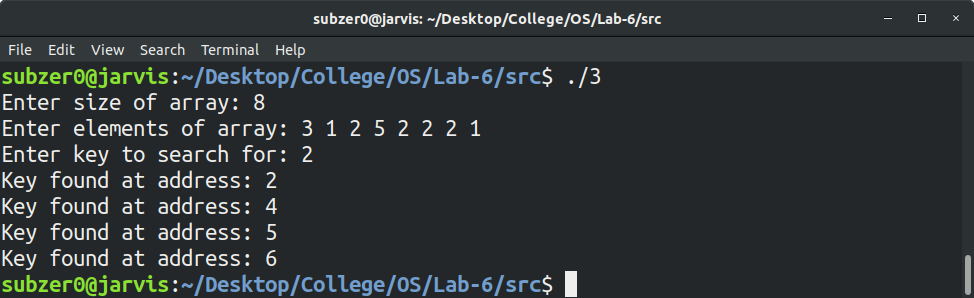
\includegraphics[width=\textwidth]{output/3.png}
\end{figure}
\bigskip


\section*{Question 4: Generation of Prime Numbers upto a limit supplied as Command Line Parameter.}
\bigskip

\par\noindent
\textbf{\Large Code: }
\smallskip
\par\noindent\rule{\textwidth}{0.4pt}
\lstinputlisting[language=c]{src/4.c}
\par\noindent\rule{\textwidth}{0.4pt}

\bigskip
\noindent
\textbf{\Large Explanation: } \\

The code above, iterates from 3 through range (user input). Every
number in this range is checked for a prime number. The check for 
each of these numbers is done by a separate thread. Hence this is 
code is parallelizable as possible.

\bigskip
\noindent
\textbf{\Large Output:}

\begin{figure}[h]
	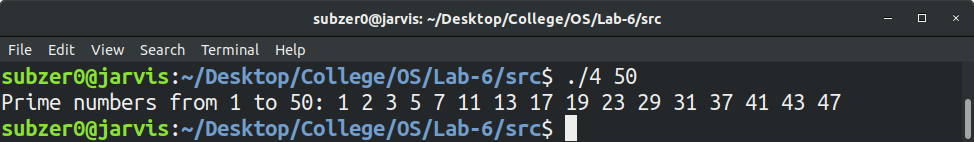
\includegraphics[width=\textwidth]{output/4.png}
\end{figure}
\bigskip

\section*{Question 5: Computation of Mean, Median, Mode for an array of integers.}
\bigskip

\par\noindent
\textbf{\Large Code: }
\smallskip
\par\noindent\rule{\textwidth}{0.4pt}
\lstinputlisting[language=c]{src/5.c}
\par\noindent\rule{\textwidth}{0.4pt}

\bigskip
\noindent
\textbf{\Large Explanation: } \\

Mean, Median and Mode are calculated in 3 separate threads. Since
threads accept the input as a void*, a structure has been created
with the array, its size, mean, median and mode as its elements.
The memory sharing feature of threads is utilised by passing the
same address to all the 3 threads. Since the threads will be 
writing to different addresses within the structure, there will be no race condition
possible.

\bigskip
\noindent
\textbf{\Large Output:}

\begin{figure}[h]
	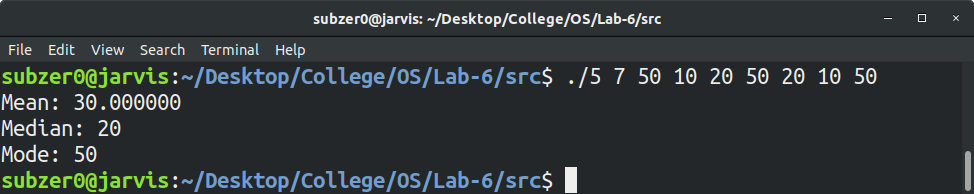
\includegraphics[width=\textwidth]{output/5.png}
\end{figure}
\bigskip

\section*{Question 6: Implement Merge Sort and Quick Sort in a multithreaded fashion.}
\bigskip

\par\noindent
\textbf{\Large Code: Merge Sort}
\smallskip
\par\noindent\rule{\textwidth}{0.4pt}
\lstinputlisting[language=c]{src/6_merge.c}
\par\noindent\rule{\textwidth}{0.4pt}

\bigskip
\noindent
\textbf{\Large Explanation: } \\

The above code is a multithreading implementation of merge sort. 
Every division is done by a new thread. Every merge is done by 
the calling thread when its child threads are complete. 

\bigskip
\noindent
\textbf{\Large Output:}

\begin{figure}[h]
	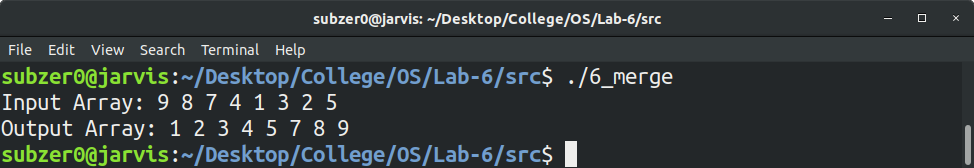
\includegraphics[width=\textwidth]{output/6_merge.png}
\end{figure}
\bigskip

\par\noindent
\textbf{\Large Code: Quick Sort}
\smallskip
\par\noindent\rule{\textwidth}{0.4pt}
\lstinputlisting[language=c]{src/6_quick.c}
\par\noindent\rule{\textwidth}{0.4pt}

\bigskip
\noindent
\textbf{\Large Explanation: } \\

The above code is a multithreading implementation of quick sort. 

\bigskip
\noindent
\textbf{\Large Output:}

\begin{figure}[h]
	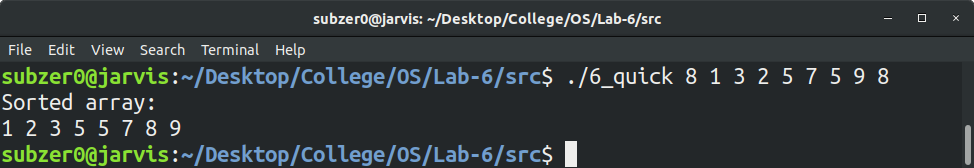
\includegraphics[width=\textwidth]{output/6_quick.png}
\end{figure}
\bigskip

\section*{Question 7: Estimation of PI Value using Monte carlo simulation technique (refer the internet for the
method..) usinreads.}
\bigskip
\bigskip

\par\noindent
\textbf{\Large Code: }
\smallskip
\par\noindent\rule{\textwidth}{0.4pt}
\lstinputlisting[language=c]{src/7.c}
\par\noindent\rule{\textwidth}{0.4pt}

\bigskip
\noindent
\textbf{\Large Explanation: } \\

Monte Carlo's estimation of PI was done in this code using threading.
4 threads are created. Each thread finds the number of points outside
and inside the circle for ITRS number of times. ITRS defines the number
of iterations that each thread runs the function. Once all threads are
complete, the estimation is completed by putting the values in the
formula.
\\\\The number of threads have been set to 4 to avoid the CPU from 
backlogging the active threads and causing the program to run 
inefficiently.

\bigskip
\noindent
\textbf{\Large Output:}

\begin{figure}[h]
	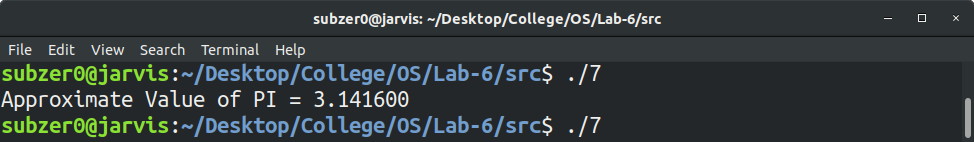
\includegraphics[width=\textwidth]{output/7.png}
\end{figure}
\bigskip

\section*{Extra Credit Questions}
\section*{Question 8: Computation of a Matrix Inverse using Determinant, Cofactor threads, etc.}
\bigskip

\par\noindent
\textbf{\Large Code: }
\smallskip
\par\noindent\rule{\textwidth}{0.4pt}
\lstinputlisting[language=c]{src/8.c}
\par\noindent\rule{\textwidth}{0.4pt}

\bigskip
\noindent
\textbf{\Large Explanation: } \\

This code is a multithreading approach of inverting a matrix. 
To find the inverse of a matrix, its determinant and adjoint 
needs to be calculated. In this code, finding the adjoint of the
matrix has been parallelized using threading. In order to avoid
the creation of a large number of threads, adjoint of every 
element in a row is calculated parallelly. So the maximum number
of threads created will be equal to number of columns. Hence the
time complexity is reduced from O($n^2$) to O($n$).


\bigskip
\noindent
\textbf{\Large Output:}

\begin{figure}[h]
	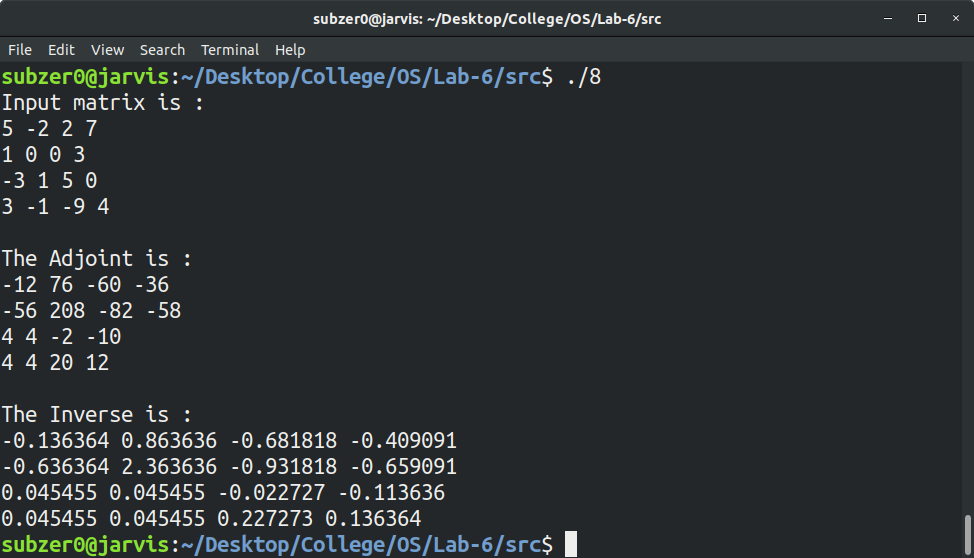
\includegraphics[width=\textwidth]{output/8.png}
\end{figure}
\bigskip

\section*{Question 9: Estimation of PI Value using Monte carlo simulation technique (refer the internet for the
method..) usinreads.}
\bigskip

Fibonacci series depends on its previous 2 elements. Hence 
whatever algo is used, to calculate the nth element, 
its previous elements have to be calculated. So, the time complexity 
can never be below O(n). \\
\\For example, to calculate $fib(7)$ from a top to bottom approach, 
we need to find $fib(6)$, $fib(5)$, ... $fib(2)$, $fib(1)$. To calculate 
$fib(6)$, we need to find $fib(5)$, $fib(4)$, ... $fib(2)$, $fib(1)$. Hence
finding all these in a linear sequential manner would lead to a 
time complexity of about O($2^n$). \\
\\Although, calculating fibonacci using a bottom up approach will take
only O($n$). \\Example: To calculate $fib(5)$, first calculate $fib(3)$
using $fib(2)$ and $fib(1)$, then calculate $fib(4)$
using $fib(3)$ and $fib(2)$ and then finally calculate $fib(5)$
using $fib(4)$ and $fib(3)$. As it can be observer, this method will take only O($n$).\\
\\Hence I feel there is no need to parallelize the top to bottom approach
requiring more hardware when the solution to the problem is just calculating
the $n^th$ fibonacci number using a bottom up approach.


\section*{Question 10: Longest common sub sequence generation problem using threads.}
\bigskip

\par\noindent
\textbf{\Large Code: }
\smallskip
\par\noindent\rule{\textwidth}{0.4pt}
\lstinputlisting[language=c]{src/10.cpp}
\par\noindent\rule{\textwidth}{0.4pt}

\bigskip
\noindent
\textbf{\Large Explanation: } \\

This program uses vectors and stl functions for speedy coding.
The program can be viewed as two parts:
1.  The first part finds all the subsequences of the first string.
2.  The second part checks if any of those subsequences matches with any subsequence of the second string.

In this program, I have multithreaded the second part. 

All subsequences of the first string are stored in a vector named 
str1\textunderscore subseq. The function check\textunderscore common\textunderscore seq takes one argument as 
a string. This function checks if there exists a subsequence in str2
which matches its argument. If such a subsequence exists, it is 
appended to a vector named common.

\pagebreak
\bigskip
\noindent
\textbf{\Large Output:}

\begin{figure}[h]
	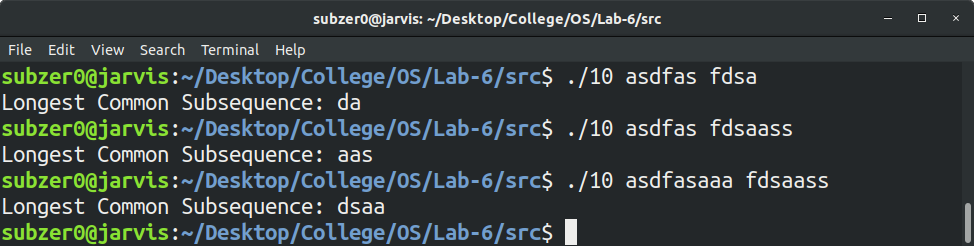
\includegraphics[width=\textwidth]{output/10.png}
\end{figure}
\bigskip

\end{document}